\section{Behavior}

\subsection{Description of Div\_unit Module}

In this section we describe what is the behaviour of div\_unit when a division or remainder operation comes from the exe\_stage at the rising edge of the cycle. 

When a new division or remainder operation arrives to the exe\_stage, request\_i signal is set to 1, and the divisor and dividend of the operation are passed through signals dvnd\_i and dvsr\_i. Exe\_stage indicates if the operation uses 64 or 32 bit operands setting int\_32\_i signal to 0 or 1 respectively. Moreover, exe\_stage indicates if the operands are signed or unsigned setting signed\_op\_i to 1 or 0 respectively.

On the first cycle div\_unit captures the operands and sets the FSM state to "FIRST". In this cycle the division unit checks if the divisor is 0, if the dividend and divisor have the same sign.

The div\_unit performs 4 steps of the long division algorithm (See Section \ref{chapter2}) on states "FIRST" and "OP". With a counter, div\_unit controls the amount of steps done. After the first 4 steps, FSM transitions from "FIRST" to "OP". When the div\_unit has done the corresponding steps for 32 or 64 bit division/remainder, the FSM transitions from "OP" to "DONE".

At "DONE" state if the divisor was a zero, quo\_o is set to "-1" and rmd\_o is set to the dividend input. Otherwise it outputs the quotient and remainder of the division.


%--------------------------------------------------------------------------------------------

\subsection{Description of Div\_4bits Module}

In this section we describe what is the behaviour of div\_4bits module.

In one cycle the div\_4bits module is performs four steps of the algorithm division. At the beginning of the cycle the div\_unit must pass the divisor, remainder and dividend\_quotient to the div\_4bits unit. In each step of the division, the divisor is always the same. However, remainder and dividend\_quotient change on each step, and must be managed by the div\_unit.The remainder contains the previous 4 step division remainder. In the first iteration this signal is set to 0. On the second iteration this signal is set to the remainder of the previous division, and so on. 

dividend\_qoutient signal encodes two variables of the division. In the first dividend\_quotient is equal to the dividend. After the first iteration div\_4bits outputs dividend\_quotient\_o, which contains on the N-4 lower bits of the dividend on the uppermost N-4 bits, while the 4 lowermost bits contain the quotient.

In Figure \ref{fig:div}, it is illustrated how dividend\_quotient signal is encoded. In this example we depict a division of 8 bits. After the first iteration the output dividend\_quotient contains on the 4 upper bits the 4 lower bits of the input dividend\_quotient. And in the 4 lower bits of the output dividend\_quotient contain the 4 upper bits of the quotient. After the second iteration, the dividend\_quotient signal contains only the quotient bits.


\begin{figure}[h]
\centering
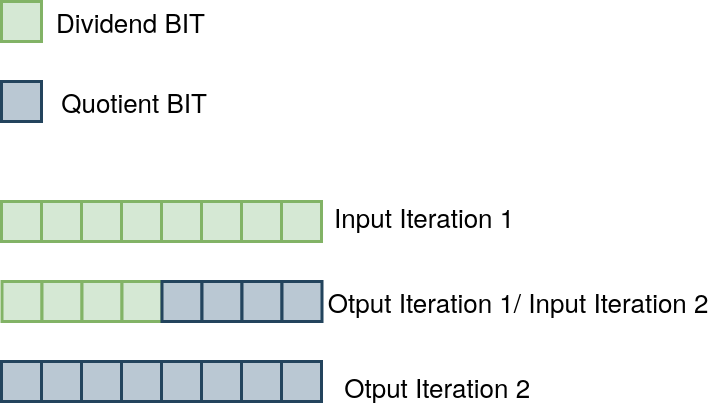
\includegraphics[width=8cm]{DIV.png}
\label{fig:div}
\end{figure}

This encoding is the result of applying the long division algorithm (See Section \ref{chapter2}). In Listing \ref{unroll} we can see the algorithm after applying a four unroll optimization and using one signal to encode dividend an quotient:

N corresponds to dividend, D to divisor, NQ to dividend\_quotient, R to remainder.

\begin{lstlisting}[label=unroll, caption=Unroll division]
NQ := N                  -- Initialize quotient and remainder to zero
R := 0                   -- Initialize remainder to zero
for i := M, M - 5, .. 0 do  -- Where n is number of bits in N 
                            -- (either 64 or 32 bits)

  R := R << 1               -- Left-shift R by 1 bit
  R(0) := NQ(64)            -- Set the least significant bit of R equal 
                            --     to the most significant bit of the dividend
  NQ := NQ << 1             -- Remove the most significant bit of the dividend
  if R >= D then
    R := R - D
    NQ(0) := 1              -- Assign 1 or 0 to the space left by the shift
  end
  
  R := R << 1               -- Left-shift R by 1 bit
  R(0) := NQ(64)            -- Set the least-significant bit of R equal 
                            --     to the most significant bit of the dividend
  NQ := NQ << 1             -- Remove the most significant bit of the dividend
  if R >= D then
    R := R - D
    NQ(0) := 1              -- Assign 1 or 0 to the space left by the shift
  end
 
  R := R << 1               -- Left-shift R by 1 bit
  R(0) := NQ(64)            -- Set the least-significant bit of R equal 
                            --     to the most significant bit of the dividend
  NQ := NQ << 1             -- Remove the most significant bit of the dividend
  if R >= D then
    R := R - D
    Q(0) := 1               -- Assign 1 or 0 to the space left by the shift
  end
  
  R := R << 1               -- Left-shift R by 1 bit
  R(0) := NQ(64)            -- Set the least-significant bit of R equal 
                            --     to the most significant bit of the dividend
  NQ := NQ << 1             -- Remove the most significant bit of the dividend
  if R >= D then
    R := R - D
    Q(0) := 1               -- Assign 1 or 0 to the space left by the shift
  end
end

\end{lstlisting}


\subsubsection{Examples}

In the following example we can see how the div\_unit performs a division and how div\_4bits is use to perform this division:

\begin{figure}[h]
\centering
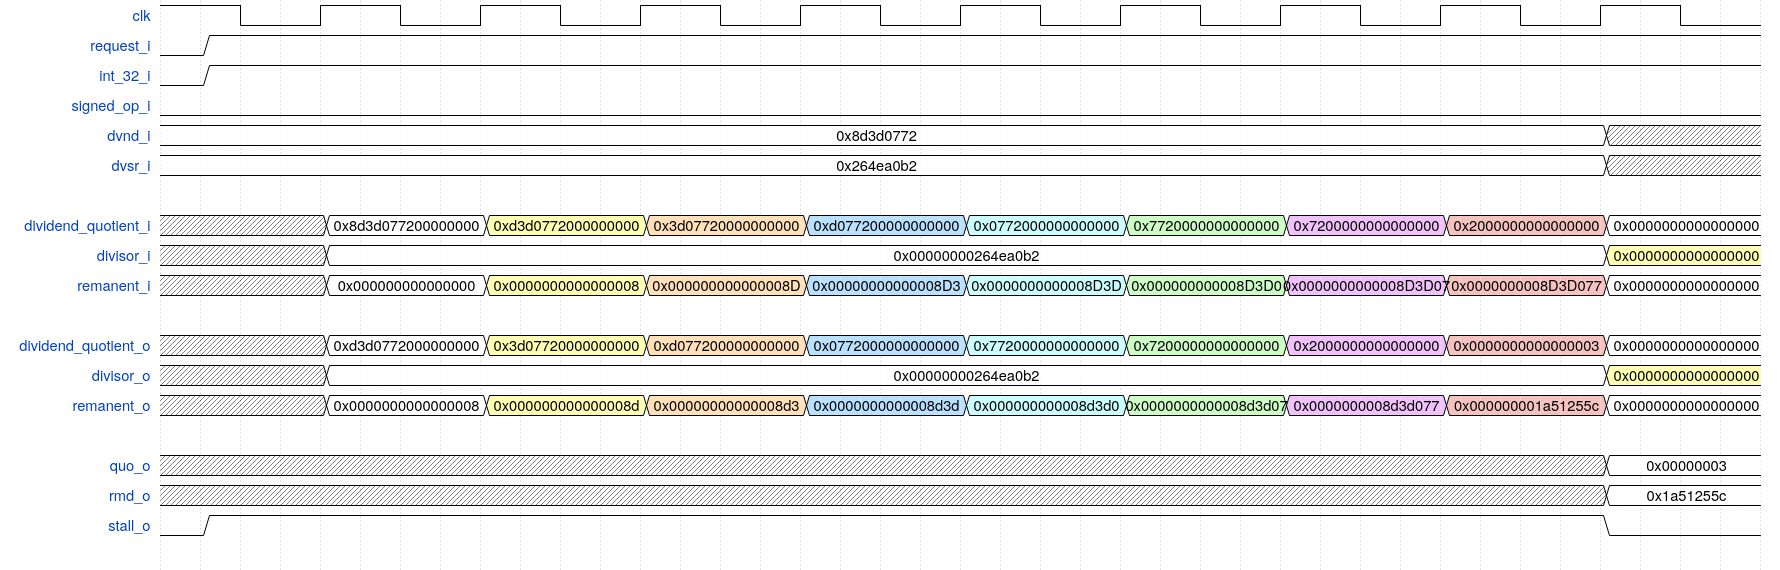
\includegraphics[width=14cm]{wave_div.png}
\end{figure}